%% bare_jrnl.tex
%% V1.4b
%% 2015/08/26
%% by Michael Shell
%% see http://www.michaelshell.org/
%% for current contact information.
%%
%% This is a skeleton file demonstrating the use of IEEEtran.cls
%% (requires IEEEtran.cls version 1.8b or later) with an IEEE
%% journal paper.
%%
%% Support sites:
%% http://www.michaelshell.org/tex/ieeetran/
%% http://www.ctan.org/pkg/ieeetran
%% and
%% http://www.ieee.org/

%%*************************************************************************
%% Legal Notice:
%% This code is offered as-is without any warranty either expressed or
%% implied; without even the implied warranty of MERCHANTABILITY or
%% FITNESS FOR A PARTICULAR PURPOSE! 
%% User assumes all risk.
%% In no event shall the IEEE or any contributor to this code be liable for
%% any damages or losses, including, but not limited to, incidental,
%% consequential, or any other damages, resulting from the use or misuse
%% of any information contained here.
%%
%% All comments are the opinions of their respective authors and are not
%% necessarily endorsed by the IEEE.
%%
%% This work is distributed under the LaTeX Project Public License (LPPL)
%% ( http://www.latex-project.org/ ) version 1.3, and may be freely used,
%% distributed and modified. A copy of the LPPL, version 1.3, is included
%% in the base LaTeX documentation of all distributions of LaTeX released
%% 2003/12/01 or later.
%% Retain all contribution notices and credits.
%% ** Modified files should be clearly indicated as such, including  **
%% ** renaming them and changing author support contact information. **
%%*************************************************************************


% *** Authors should verify (and, if needed, correct) their LaTeX system  ***
% *** with the testflow diagnostic prior to trusting their LaTeX platform ***
% *** with production work. The IEEE's font choices and paper sizes can   ***
% *** trigger bugs that do not appear when using other class files.       ***                          ***
% The testflow support page is at:
% http://www.michaelshell.org/tex/testflow/



\documentclass[journal]{IEEEtran}
%
% If IEEEtran.cls has not been installed into the LaTeX system files,
% manually specify the path to it like:
% \documentclass[journal]{../sty/IEEEtran}


\usepackage{url}
\usepackage{graphicx}
\usepackage{float}
\usepackage{subfig}
\usepackage{algorithm}  
\usepackage{algpseudocode}  
\usepackage{amsmath}  
\renewcommand{\algorithmicrequire}{\textbf{Input:}}  % Use Input in the format of Algorithm  
\renewcommand{\algorithmicensure}{\textbf{Output:}} % Use Output in the format of Algorithm
\newcommand*{\Break}{\textbf{break}}
\usepackage{booktabs}
\usepackage{array}
\usepackage{wrapfig}
\usepackage{amsfonts}
\usepackage{epstopdf}
\usepackage{makecell}
\usepackage{caption}
\newcommand{\subsubsubsection}[1]{\paragraph{#1}\mbox{}\\}
\setcounter{secnumdepth}{4} % how many sectioning levels to assign numbers to
\setcounter{tocdepth}{4} % how many sectioning levels to show in ToC

% Some very useful LaTeX packages include:
% (uncomment the ones you want to load)


% *** MISC UTILITY PACKAGES ***
%
%\usepackage{ifpdf}
% Heiko Oberdiek's ifpdf.sty is very useful if you need conditional
% compilation based on whether the output is pdf or dvi.
% usage:
% \ifpdf
%   % pdf code
% \else
%   % dvi code
% \fi
% The latest version of ifpdf.sty can be obtained from:
% http://www.ctan.org/pkg/ifpdf
% Also, note that IEEEtran.cls V1.7 and later provides a builtin
% \ifCLASSINFOpdf conditional that works the same way.
% When switching from latex to pdflatex and vice-versa, the compiler may
% have to be run twice to clear warning/error messages.






% *** CITATION PACKAGES ***
%
%\usepackage{cite}
% cite.sty was written by Donald Arseneau
% V1.6 and later of IEEEtran pre-defines the format of the cite.sty package
% \cite{} output to follow that of the IEEE. Loading the cite package will
% result in citation numbers being automatically sorted and properly
% "compressed/ranged". e.g., [1], [9], [2], [7], [5], [6] without using
% cite.sty will become [1], [2], [5]--[7], [9] using cite.sty. cite.sty's
% \cite will automatically add leading space, if needed. Use cite.sty's
% noadjust option (cite.sty V3.8 and later) if you want to turn this off
% such as if a citation ever needs to be enclosed in parenthesis.
% cite.sty is already installed on most LaTeX systems. Be sure and use
% version 5.0 (2009-03-20) and later if using hyperref.sty.
% The latest version can be obtained at:
% http://www.ctan.org/pkg/cite
% The documentation is contained in the cite.sty file itself.






% *** GRAPHICS RELATED PACKAGES ***
%
\ifCLASSINFOpdf
% \usepackage[pdftex]{graphicx}
% declare the path(s) where your graphic files are
% \graphicspath{{../pdf/}{../jpeg/}}
% and their extensions so you won't have to specify these with
% every instance of \includegraphics
% \DeclareGraphicsExtensions{.pdf,.jpeg,.png}
\else
% or other class option (dvipsone, dvipdf, if not using dvips). graphicx
% will default to the driver specified in the system graphics.cfg if no
% driver is specified.
% \usepackage[dvips]{graphicx}
% declare the path(s) where your graphic files are
% \graphicspath{{../eps/}}
% and their extensions so you won't have to specify these with
% every instance of \includegraphics
% \DeclareGraphicsExtensions{.eps}
\fi
% graphicx was written by David Carlisle and Sebastian Rahtz. It is
% required if you want graphics, photos, etc. graphicx.sty is already
% installed on most LaTeX systems. The latest version and documentation
% can be obtained at: 
% http://www.ctan.org/pkg/graphicx
% Another good source of documentation is "Using Imported Graphics in
% LaTeX2e" by Keith Reckdahl which can be found at:
% http://www.ctan.org/pkg/epslatex
%
% latex, and pdflatex in dvi mode, support graphics in encapsulated
% postscript (.eps) format. pdflatex in pdf mode supports graphics
% in .pdf, .jpeg, .png and .mps (metapost) formats. Users should ensure
% that all non-photo figures use a vector format (.eps, .pdf, .mps) and
% not a bitmapped formats (.jpeg, .png). The IEEE frowns on bitmapped formats
% which can result in "jaggedy"/blurry rendering of lines and letters as
% well as large increases in file sizes.
%
% You can find documentation about the pdfTeX application at:
% http://www.tug.org/applications/pdftex





% *** MATH PACKAGES ***
%
%\usepackage{amsmath}
% A popular package from the American Mathematical Society that provides
% many useful and powerful commands for dealing with mathematics.
%
% Note that the amsmath package sets \interdisplaylinepenalty to 10000
% thus preventing page breaks from occurring within multiline equations. Use:
%\interdisplaylinepenalty=2500
% after loading amsmath to restore such page breaks as IEEEtran.cls normally
% does. amsmath.sty is already installed on most LaTeX systems. The latest
% version and documentation can be obtained at:
% http://www.ctan.org/pkg/amsmath





% *** SPECIALIZED LIST PACKAGES ***
%
%\usepackage{algorithmic}
% algorithmic.sty was written by Peter Williams and Rogerio Brito.
% This package provides an algorithmic environment fo describing algorithms.
% You can use the algorithmic environment in-text or within a figure
% environment to provide for a floating algorithm. Do NOT use the algorithm
% floating environment provided by algorithm.sty (by the same authors) or
% algorithm2e.sty (by Christophe Fiorio) as the IEEE does not use dedicated
% algorithm float types and packages that provide these will not provide
% correct IEEE style captions. The latest version and documentation of
% algorithmic.sty can be obtained at:
% http://www.ctan.org/pkg/algorithms
% Also of interest may be the (relatively newer and more customizable)
% algorithmicx.sty package by Szasz Janos:
% http://www.ctan.org/pkg/algorithmicx




% *** ALIGNMENT PACKAGES ***
%
%\usepackage{array}
% Frank Mittelbach's and David Carlisle's array.sty patches and improves
% the standard LaTeX2e array and tabular environments to provide better
% appearance and additional user controls. As the default LaTeX2e table
% generation code is lacking to the point of almost being broken with
% respect to the quality of the end results, all users are strongly
% advised to use an enhanced (at the very least that provided by array.sty)
% set of table tools. array.sty is already installed on most systems. The
% latest version and documentation can be obtained at:
% http://www.ctan.org/pkg/array


% IEEEtran contains the IEEEeqnarray family of commands that can be used to
% generate multiline equations as well as matrices, tables, etc., of high
% quality.




% *** SUBFIGURE PACKAGES ***
%\ifCLASSOPTIONcompsoc
%  \usepackage[caption=false,font=normalsize,labelfont=sf,textfont=sf]{subfig}
%\else
%  \usepackage[caption=false,font=footnotesize]{subfig}
%\fi
% subfig.sty, written by Steven Douglas Cochran, is the modern replacement
% for subfigure.sty, the latter of which is no longer maintained and is
% incompatible with some LaTeX packages including fixltx2e. However,
% subfig.sty requires and automatically loads Axel Sommerfeldt's caption.sty
% which will override IEEEtran.cls' handling of captions and this will result
% in non-IEEE style figure/table captions. To prevent this problem, be sure
% and invoke subfig.sty's "caption=false" package option (available since
% subfig.sty version 1.3, 2005/06/28) as this is will preserve IEEEtran.cls
% handling of captions.
% Note that the Computer Society format requires a larger sans serif font
% than the serif footnote size font used in traditional IEEE formatting
% and thus the need to invoke different subfig.sty package options depending
% on whether compsoc mode has been enabled.
%
% The latest version and documentation of subfig.sty can be obtained at:
% http://www.ctan.org/pkg/subfig




% *** FLOAT PACKAGES ***
%
%\usepackage{fixltx2e}
% fixltx2e, the successor to the earlier fix2col.sty, was written by
% Frank Mittelbach and David Carlisle. This package corrects a few problems
% in the LaTeX2e kernel, the most notable of which is that in current
% LaTeX2e releases, the ordering of single and double column floats is not
% guaranteed to be preserved. Thus, an unpatched LaTeX2e can allow a
% single column figure to be placed prior to an earlier double column
% figure.
% Be aware that LaTeX2e kernels dated 2015 and later have fixltx2e.sty's
% corrections already built into the system in which case a warning will
% be issued if an attempt is made to load fixltx2e.sty as it is no longer
% needed.
% The latest version and documentation can be found at:
% http://www.ctan.org/pkg/fixltx2e


%\usepackage{stfloats}
% stfloats.sty was written by Sigitas Tolusis. This package gives LaTeX2e
% the ability to do double column floats at the bottom of the page as well
% as the top. (e.g., "\begin{figure}[!b]" is not normally possible in
	% LaTeX2e). It also provides a command:
	%\fnbelowfloat
	% to enable the placement of footnotes below bottom floats (the standard
	% LaTeX2e kernel puts them above bottom floats). This is an invasive package
	% which rewrites many portions of the LaTeX2e float routines. It may not work
	% with other packages that modify the LaTeX2e float routines. The latest
	% version and documentation can be obtained at:
	% http://www.ctan.org/pkg/stfloats
	% Do not use the stfloats baselinefloat ability as the IEEE does not allow
	% \baselineskip to stretch. Authors submitting work to the IEEE should note
	% that the IEEE rarely uses double column equations and that authors should try
	% to avoid such use. Do not be tempted to use the cuted.sty or midfloat.sty
	% packages (also by Sigitas Tolusis) as the IEEE does not format its papers in
	% such ways.
	% Do not attempt to use stfloats with fixltx2e as they are incompatible.
	% Instead, use Morten Hogholm'a dblfloatfix which combines the features
	% of both fixltx2e and stfloats:
	%
	% \usepackage{dblfloatfix}
	% The latest version can be found at:
	% http://www.ctan.org/pkg/dblfloatfix
	
	
	
	
	%\ifCLASSOPTIONcaptionsoff
	%  \usepackage[nomarkers]{endfloat}
	% \let\MYoriglatexcaption\caption
	% \renewcommand{\caption}[2][\relax]{\MYoriglatexcaption[#2]{#2}}
	%\fi
	% endfloat.sty was written by James Darrell McCauley, Jeff Goldberg and 
	% Axel Sommerfeldt. This package may be useful when used in conjunction with 
	% IEEEtran.cls'  captionsoff option. Some IEEE journals/societies require that
	% submissions have lists of figures/tables at the end of the paper and that
	% figures/tables without any captions are placed on a page by themselves at
	% the end of the document. If needed, the draftcls IEEEtran class option or
	% \CLASSINPUTbaselinestretch interface can be used to increase the line
	% spacing as well. Be sure and use the nomarkers option of endfloat to
	% prevent endfloat from "marking" where the figures would have been placed
	% in the text. The two hack lines of code above are a slight modification of
	% that suggested by in the endfloat docs (section 8.4.1) to ensure that
	% the full captions always appear in the list of figures/tables - even if
	% the user used the short optional argument of \caption[]{}.
	% IEEE papers do not typically make use of \caption[]'s optional argument,
	% so this should not be an issue. A similar trick can be used to disable
	% captions of packages such as subfig.sty that lack options to turn off
	% the subcaptions:
	% For subfig.sty:
	% \let\MYorigsubfloat\subfloat
	% \renewcommand{\subfloat}[2][\relax]{\MYorigsubfloat[]{#2}}
	% However, the above trick will not work if both optional arguments of
	% the \subfloat command are used. Furthermore, there needs to be a
	% description of each subfigure *somewhere* and endfloat does not add
	% subfigure captions to its list of figures. Thus, the best approach is to
	% avoid the use of subfigure captions (many IEEE journals avoid them anyway)
	% and instead reference/explain all the subfigures within the main caption.
	% The latest version of endfloat.sty and its documentation can obtained at:
	% http://www.ctan.org/pkg/endfloat
	%
	% The IEEEtran \ifCLASSOPTIONcaptionsoff conditional can also be used
	% later in the document, say, to conditionally put the References on a 
	% page by themselves.
	
	
	
	
	% *** PDF, URL AND HYPERLINK PACKAGES ***
	%
	%\usepackage{url}
	% url.sty was written by Donald Arseneau. It provides better support for
	% handling and breaking URLs. url.sty is already installed on most LaTeX
	% systems. The latest version and documentation can be obtained at:
	% http://www.ctan.org/pkg/url
	% Basically, \url{my_url_here}.
	
	
	
	
	% *** Do not adjust lengths that control margins, column widths, etc. ***
	% *** Do not use packages that alter fonts (such as pslatex).         ***
	% There should be no need to do such things with IEEEtran.cls V1.6 and later.
	% (Unless specifically asked to do so by the journal or conference you plan
	% to submit to, of course. )
	
	
	% correct bad hyphenation here
	\hyphenation{op-tical net-works semi-conduc-tor}
	
	
	\begin{document}
		%
		% paper title
		% Titles are generally capitalized except for words such as a, an, and, as,
		% at, but, by, for, in, nor, of, on, or, the, to and up, which are usually
		% not capitalized unless they are the first or last word of the title.
		% Linebreaks \\ can be used within to get better formatting as desired.
		% Do not put math or special symbols in the title.
		\title{Survey of Intelligent Archaeology}
		%
		%
		% author names and IEEE memberships
		% note positions of commas and nonbreaking spaces ( ~ ) LaTeX will not break
		% a structure at a ~ so this keeps an author's name from being broken across
		% two lines.
		% use \thanks{} to gain access to the first footnote area
		% a separate \thanks must be used for each paragraph as LaTeX2e's \thanks
		% was not built to handle multiple paragraphs
		%
		
		\author{Lin~Yuhang, Peng Shubo}% <-this % stops a space
		
		
		% note the % following the last \IEEEmembership and also \thanks - 
		% these prevent an unwanted space from occurring between the last author name
		% and the end of the author line. i.e., if you had this:
		% 
		% \author{....lastname \thanks{...} \thanks{...} }
		%                     ^------------^------------^----Do not want these spaces!
		%
		% a space would be appended to the last name and could cause every name on that
		% line to be shifted left slightly. This is one of those "LaTeX things". For
		% instance, "\textbf{A} \textbf{B}" will typeset as "A B" not "AB". To get
		% "AB" then you have to do: "\textbf{A}\textbf{B}"
		% \thanks is no different in this regard, so shield the last } of each \thanks
	% that ends a line with a % and do not let a space in before the next \thanks.
	% Spaces after \IEEEmembership other than the last one are OK (and needed) as
	% you are supposed to have spaces between the names. For what it is worth,
	% this is a minor point as most people would not even notice if the said evil
	% space somehow managed to creep in.
	
	
	
	% The paper headers
	\markboth{Lin~Yuhang, Peng~Shubo, December~2022}%
	{Shell \MakeLowercase{\textit{et al.}}: Bare Demo of IEEEtran.cls for IEEE Journals}
	% The only time the second header will appear is for the odd numbered pages
	% after the title page when using the twoside option.
	% 
	% *** Note that you probably will NOT want to include the author's ***
	% *** name in the headers of peer review papers.                   ***
	% You can use \ifCLASSOPTIONpeerreview for conditional compilation here if
	% you desire.
	
	
	
	
	% If you want to put a publisher's ID mark on the page you can do it like
	% this:
	%\IEEEpubid{0000--0000/00\$00.00~\copyright~2015 IEEE}
	% Remember, if you use this you must call \IEEEpubidadjcol in the second
	% column for its text to clear the IEEEpubid mark.
	
	
	
	% use for special paper notices
	%\IEEEspecialpapernotice{(Invited Paper)}
	
	
	
	
	% make the title area
	\maketitle
	
	% As a general rule, do not put math, special symbols or citations
	% in the abstract or keywords.
	\begin{abstract}
		Recently more and more AI techniques are used in archaeology area, one of which is machine learning (ML). Application of ML can be divided into two main categories: object classification and site searching. Classification can not only be used to classify fragments, like pottery or papyrus, but also help to merge messy fragments into complete patterns. Site searching is a new topic raise recently thanks to the popularity of satellites, whose generated systematized data offers premises for ML. But ML still has some shortage, most of which limited by nature of archaeology. In future, ML maybe more used in identification of archaeological sites, or illegal treatment about art products. 
	\end{abstract}
	
	% Note that keywords are not normally used for peerreview papers.
	\begin{IEEEkeywords}
		Archaeology, machine learning, classification, site searching.
	\end{IEEEkeywords}
	
	
	
	
	
	
	% For peer review papers, you can put extra information on the cover
	% page as needed:
	% \ifCLASSOPTIONpeerreview
	% \begin{center} \bfseries EDICS Category: 3-BBND \end{center}
	% \fi
	%
	% For peerreview papers, this IEEEtran command inserts a page break and
	% creates the second title. It will be ignored for other modes.
	\IEEEpeerreviewmaketitle
	
	
	
	\section{Introduction}
	% The very first letter is a 2 line initial drop letter followed
	% by the rest of the first word in caps.
	% 
	% form to use if the first word consists of a single letter:
	% \IEEEPARstart{A}{demo} file is ....
	% 
	% form to use if you need the single drop letter followed by
	% normal text (unknown if ever used by the IEEE):
	% \IEEEPARstart{A}{}demo file is ....
	% 
	% Some journals put the first two words in caps:
	% \IEEEPARstart{T}{his demo} file is ....
	% 
	% Here we have the typical use of a "T" for an initial drop letter
	% and "HIS" in caps to complete the first word.
	\IEEEPARstart {A}{rtificial} Intelligence (AI for short) is a new study area rising in recent centuries, and can be divided into several directions, like Machine Learning (ML) or Neural Network (NN). Five to ten years ago, they were concepts unknown to archaeologists. But now, AI is widely used, there are even sessions dedicated to AI at archaeological conferences.\cite{heritage4010008}
	
	ML is programming allowing algorithm learning from data and adjust its parameters and then make predictions on new data. Objects must be quantify into digital data first and can be any type, like sonar data under water\cite{Drap2018UnderwaterPF} or aerial
	laser scanning data \cite{rs10020225}. ML uses mathematical techniques to analyze a set of already-classified objects and generate "classifiers" for each category. In theory, objects in every category is identified from other categories in mathematics. In short, ML use math to classify quantifiable objects into different groups.\cite{bickler_2021}
	
	Ml application can be divided into two main types: classify archaeological objects, and identify archaeological sites, both of which will be explained more detailed in \ref{application}. 
	
	Deep learning(DL) a branch of ML, the biggest difference is that, ML needs human to appoint characteristics of object to be trained, while DL do not need pre-appointed characteristics. What DL processing is a large number of data, and DL can learn and choose significant characteristics by itself. DL will first determine which characteristics are related to its goal, then attempt to obtain accessible features on layer level, finally determine which accessible features match its goal best.
	
	
	\section{Application}\label{application}

	DL has been successfully used in many applications. Among the DL
	methods, recurrent neural networks (RNNs) are good at dealing with sequential data as they
	take into account temporal information. RNNs have been applied in speech recognition to
	map acoustic sequences to phonetic sequences. RNNs have also been used in natural
	language processing to translate text from one language to another. Another
	famous method in DL is convolutional neural networks (CNNs). CNNs take into
	account spatial correlation among data points and hence perform well in image-based data.
	CNNs have been used in image classification, face recognition,
	scene labelling, and so on. DL methods are also used in the field of remote sensing.
	For example, Hu and Yuan used CNNs to extract digital terrain models (DTMs) and filter out non-ground
	points from airborne laser scanning (ALS) data, which was claimed that this method performs better than
	previous filtering methods\cite{HuXiangyun2016DCfD}.

	In the papers we've read, we've found that all of them, without exception, use CNNs to study a specific thing.
	This is because the things they studied were all based on image data, in which CNNs performs better than RNNs.

	We divide the papers that use CNNs into two types: one is to classify archaeological objects like papyrus, potteries, and so on, the other is to detect objects in archaeological sites.

	\subsection{classify archaeological objects}

	\begin{itemize}
	\item In the paper\cite{Papyrus}, a method is proposed for matching and assembling pairs of ancient papyrus fragments containing mostly unknown scriptures.
		  This task, which is assembling fragments in a puzzle-like manner into a composite picture, plays an important role in the archaeology, because it can help historic artifacts to reconstruct archaeological objects for research.
		  The proposed method is to use image processing and machine learning techniques to identify matching fragments, and then support the quick and automated classification of matching pairs of papyrus fragments as well
		  as the geometric alignment of the pairs against each other. The algorithm was trained on a batch of fragments which was excavated from the Dead Sea caves and is dated circa the 1st
		  century BCE. The algorithm shows excellent results on a validation set which is of a similar origin and conditions.
		  Then the algorithm was used to  against a real-life set of fragments for with no prior knowledge or labeling of matches.
		  This test batch is considered extremely challenging due to its poor condition and the small size of its fragments. Evidently,
		  numerous researchers have tried seeking matches within this batch with very little success. The algorithm performance on
		  this batch was sub-optimal, returning a relatively large ratio of false positives. However, the results showed that this algorithm
		  eliminated 98\% of the possible matches thus reducing the amount of work needed for manual inspection, which means this algorithm was quite useful. Indeed, experts that
		  reviewed the results have identified some positive matches as potentially true and referred them for further investigation.
		  \begin{figure}[htbp]
			\centering
			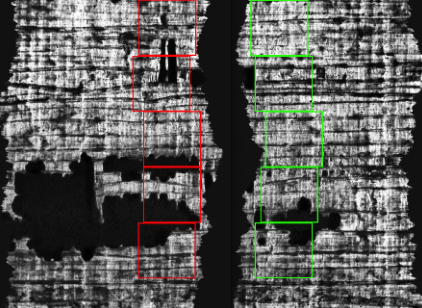
\includegraphics[width=0.9\linewidth]{./picture/fig1.png}
			\caption{An example of two adjacent artificially torn fragments with a set of candidate squares to be used in
			the matching phase.}
		  \end{figure}
	\item In the paper\cite{Syrian_images}, the project developed at Dumbarton Oaks---a research institute and library, museum, and historic 
		  garden affiliated with Harvard University and located in Washington, DC--- focused on a 
		  collection of 10,000 images of Syrian monuments in the institution's Image Collections and 
		  Fieldwork Archives (ICFA). Drawing on that project, as well as the broader landscape of AI-based categorisation efforts in the fields of art and architecture, authors' insights on the potential of AI to facilitate and enhance archival image access and recording will be shaerd. Many of the Syrian sites in the Dumbarton Oaks collection have been inaccessible to researchers and the public for over a decade and/or have been damaged or destroyed. For Dumbarton Oaks, the primary goal was to explore whether AI can improve the speed and efficiency of sharing collections and allow for more sophisticated curation by subject experts who, thanks to automation, would be relieved of the burden of rote processing. The methods and techniques explored included multi-label classification, multi-task classification, unsupervised image clustering, and explainability.
		  \begin{figure}[htbp]
			\centering
			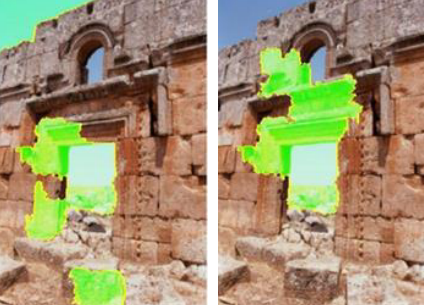
\includegraphics[width=0.9\linewidth]{./picture/fig2.png}
			\caption{Explainability heatmaps for predictions of the 
			classes “architecture” (left) and “façades” (right) by the 
			Phase 1 classifier.}
		  \end{figure}
	\item The main contribution in this paper\cite{heritage4010008} is the completion of the project called ArchAIDE.
		  This project  realised an AI-based application to recognise archaeological pottery.
		  Pottery is of paramount importance for understanding archaeological contexts. However, recognition of
		  ceramics is still a manual, time-consuming activity , reliant on analogue catalogues. The project
		  developed two complementary machine-learning tools to propose identifications based on images
		  captured on-site, for optimising and economising this process, while retaining key decision points
		  necessary to create trusted results. One method relies on the shape of a potsherd; the other is based
		  on decorative features. For the shape-based recognition, a novel deep-learning architecture was
		  employed, integrating shape information from points along the inner and outer profile of a sherd.
		  The decoration classifier is based on relatively standard architectures used in image recognition. In
		  both cases, training the algorithms meant facing challenges related to real-world archaeological data:
		  the scarcity of labelled data; extreme imbalance between instances of different categories; and the
		  need to take note of minute differentiating features. Finally , the creation of a desktop and mobile
		  application that integrates the AI classifiers provides an easy-to-use interface for pottery classification
		  and storing pottery data.
		  
		  In particular, since this project ArchAIDE is the most classic and mature one among all paper, the more detailed and overall explanation will be given in \ref{example}.
		  \begin{figure}[htbp]
			\centering
			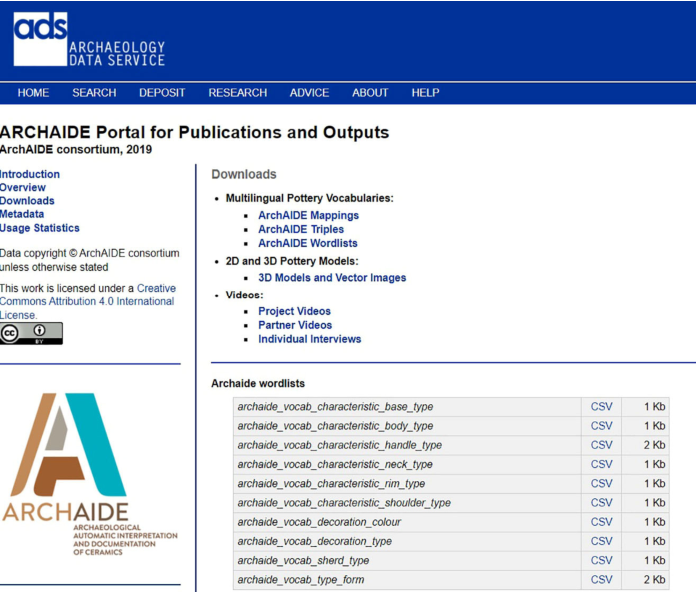
\includegraphics[width=0.9\linewidth]{./picture/fig3.png}
			\caption{The ArchAIDE portal is available at the Archaeology Data Service of the University of York.}
		  \end{figure}
		  \begin{figure}[htbp]
			\centering
			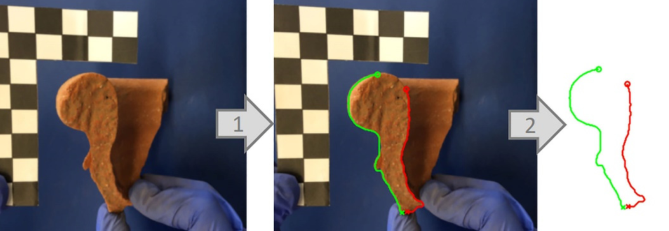
\includegraphics[width=0.9\linewidth]{./picture/fig4.png}
			\caption{The automated extraction of the outer (green) and inner (red) profiles from a real-world sherd image.}
		  \end{figure}
	\item The paper\cite{CeramicFabric} indicate that deep learning with CNNs is a highly accessible and 
	      effective method for classifying ceramic fabrics based on images of petrographic thin 
		  sections and that it can likely be applied on a larger scale.
		  Classification of ceramic fabrics has long held a major role in archaeological pursuits. 
		  It helps answer research questions related to ceramic technology, provenance, and 
		  exchange and provides an overall deeper understanding of the ceramic material at 
		  hand. One of the most effective means of classification is through petrographic thin 
		  section analysis. However, ceramic petrography is a difficult and often tedious task 
		  that requires direct observation and sorting by domain experts. In this paper, a deep 
		  learning model is built to automatically recognize and classify ceramic fabrics, which 
		  expedites the process of classification and lessens the requirements on experts. The 
		  samples consist of images of petrographic thin sections under cross-polarized light 
		  originating from the Cocal-period (AD 1000-1525) archaeological site of Guadalupe 
		  on the northeast coast of Honduras. Two CNNs, 
		  VGG19 and ResNet50, are compared against each other using two approaches to 
		  partitioning training, validation, and testing data. The technique employs a standard 
		  transfer learning process whereby the bottom layers of the CNNs are pre-trained 
		  on the ImageNet dataset and frozen, while a single pooling layer and three dense 
		  layers are added to 'tune' the model to the thin section dataset. After selecting fabric 
		  groups with at least three example sherds each, the technique can classify thin section 
		  images into one of five fabric groups with over 93\% accuracy in each of four tests. 
		  \begin{figure}[htbp]
			\centering
			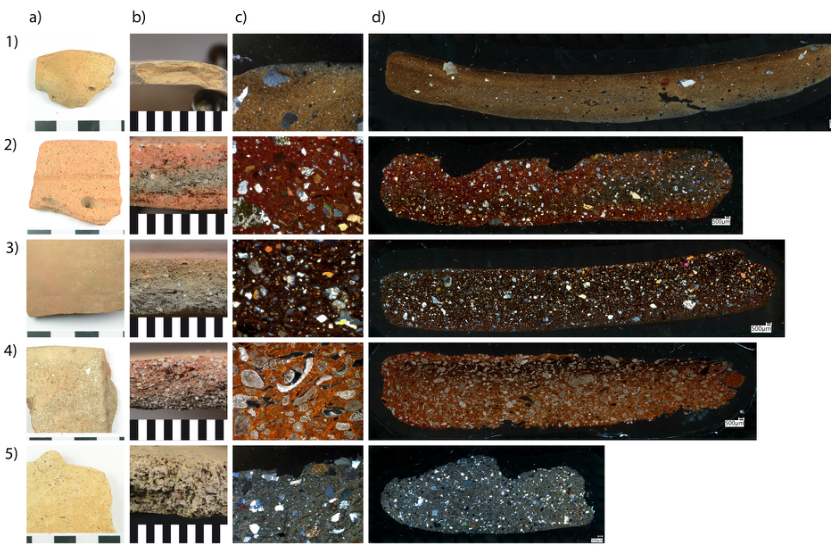
\includegraphics[width=1.0\linewidth]{./picture/fig5.png}
			\caption{Examples of the five ceramic fabric types analyzed.}
		  \end{figure}
	\item In the study\cite{PawlowiczLeszekM.2021Aodl}, an alternate approach to archaeological typology which uses DL to classify digital 
		  images of decorated pottery sherds into an existing typological framework is presented. This study focuses on a specific kind of ancient painted pottery from the American Southwest, Tusayan White Ware (TWW), but it is believed that it has broader implications for a wide range of geographical settings and artifact types. The results show that when properly trained, a deep learning model can assign types to digital images of decorated sherds with an accuracy comparable to, and sometimes higher than, four expert-level contemporary archaeologists. The technique also offers novel tools for visualizing both the importance of diagnostic design elements and overall design relationships between groups of pottery sherds. This method can objectively match a specific unclassified sherd image to its most similar counterparts through a search of thousands of digital photos. This discovery has important archaeological implications for analyzing time relationships, monitoring stylistic trends, reconstructing fragmentary artifacts, identifying ancient artisans, and studying the evolution and spread of ancient technologies and styles. It also shows how deep learning models can potentially supplement or supplant traditional typologies in favor of more direct groupings and comparisons of artifacts.
		  \begin{figure}[htbp]
			\centering
			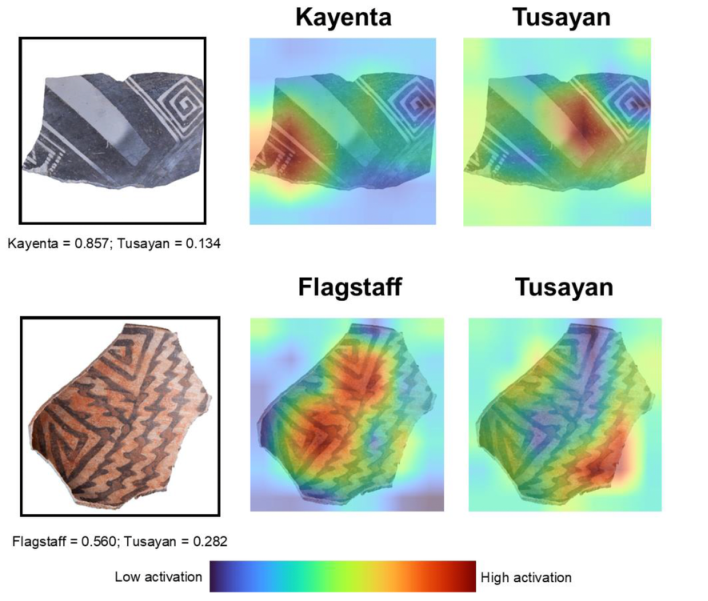
\includegraphics[width=1.0\linewidth]{./picture/fig6.png}
			\caption{ Grad-CAM heat maps for TWW sherds, showing areas of high (red) and low (blue) model activation for a Kayenta sherd (top) and Flagstaff sherd (bottom). 
			CNN-model-calculated type confidences shown below each sherd.}
		  \end{figure}
	\end{itemize}

	\subsection{detect objects in archaeological sites}

	Airborne laser scanning (ALS) is of great use in
	collecting and documenting detailed measurements from an area of interest. However, it is
	time consuming for scientists to manually analyze the collected ALS data. One possible way to
	automate this process is using deep neural networks.

	In the paper\cite{AOD}, a hierarchical CNN model is builded to detect objects in archaeological sites
	using digital terrain models (DTMs) generated from ALS data. 
	The	data is acquired from the Harz mining Region in Lower Saxony, where a high density of different
	archaeological monuments including the UNESCO world heritage site Historic Town of Goslar,
	Mines of Rammelsberg, and the Upper Harz Water Management System can be found. Objects to be detected are archaeological
	objects such as hollow ways, streams, pathways, lakes, streets, ditches, heaps, mining shafts,
	and more, but for this study, the model is fit to detect 4 classes of objects: natural streams, lakes, tracks, and an 'others' class
	which represents the rest of the objects for which enough labeled data is not available yet. To
	compare and validate the method in this paper, some experiments on the same data set using two existing
	deep learning models were conducted. The first model is VGG-16; an image classification network pretrained
	on ImageNet data. The second model is a stacked autoencoders model. The results of the
	classification as analyzed in this paper show that our model is suitably tuned for this task as it
	achieves the best classification accuracy of around 91 percent, compared to 88 percent and 82
	percent accuracy by the pretrained and stacked autoencoders models, respectively.
	\begin{figure}[htbp]
		\centering
		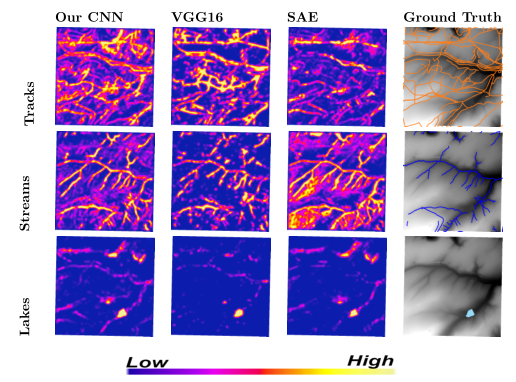
\includegraphics[width=1.0\linewidth]{./picture/fig7.png}
		\caption{Heat maps using filter size 48 x 48. Colors show the confidence of the models in detecting
		objects at that location.}
	  \end{figure}
	  \begin{figure}[htbp]
		\centering
		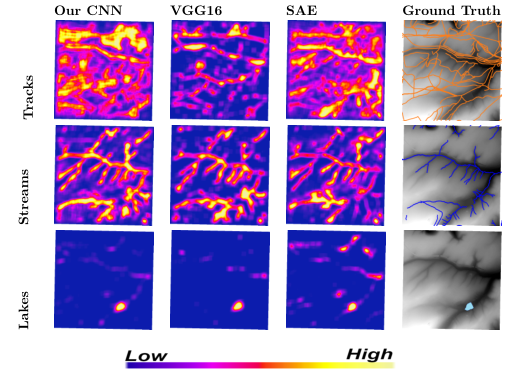
\includegraphics[width=1.0\linewidth]{./picture/fig8.png}
		\caption{Heat maps using filter size 98 x 98. Colors show the confidence of the models in detecting
		objects at that location.}
	  \end{figure}

	\subsection{More}

	We believe that there are many other studies using RNNs to study the meaning of certain patterns on ancient artifacts or to try to decipher ancient texts.
	But this is out of the scope of our survey.
	
	\section{ArchAIDE Project}\label{example}
	
	To make things clear, a classic and mature classification project is briefly shown in this part. The reason why classification is chosen rather than searching sites is that, the number of paper about classification is much more than searching area. Among all applications in paper, the most classic and the most mature one is picked out here. 
	
	The name of project introduced here is ``ArchAIDE''. The most remarkable characteristic of this project is that, it not only invent algorithm and do analysis on data from both view of shape and decorations, but also realize a system that could have a realworld implementation. 
	
	\subsection{General Introduction}
	
	ArchAIDE project aims at optimizing the ceramic identification process. It developed two different deep neural networks to recognize pottery through images using a mobile device.The first network is specially used for image recognition, also called appearance-based recognition. The second network uses the shape of fragmentation to identify. 
	
	Unlike familiar worries about AI, ArchAIDE will not replace the knowledge of domain specialists. On the contrary, it put archaeologists' role in the center of decision-making process in the identification workflow, which can be seen in \ref{method}.
	
	\subsection{Materials}
	
	A correct result of classification relies on two parts: the label or the name of each category, and the available data for both shape-based and appearance-based recognition. But first, the class of relics should be determined.
	
	\subsubsection{Classes for training}
	\ 
	
	Among all categories of cultural relics, the project choose four realworld classes for training:
	
	\begin{itemize}
		\item Amphorae manufactured throughout the Roman world between the late 3rd century BCE and the early 7th century CE. (Figure \ref{roman})
		\item Roman Terra Sigillata manufactured in Italy , Spain, and South Gaul between the 1st century BCE and the 3rd century CE.
		\item Majolica produced in Montelupo Fiorentino (Italy) between 14th and 18th century.
		\item medieval and post-medieval Majolica from Barcelona and Valencia. (Figure \ref{majolica})
	\end{itemize}
	
	\begin{figure}[htbp]%
		\centering
		\subfloat[Roman amphorae]{
			\label{roman}
			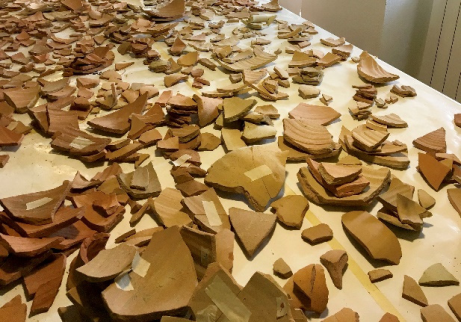
\includegraphics[width=0.45\linewidth]{./picture/material1.png}
		}\hfill
		\subfloat[Majolica of Montelupo Fiorentino]{
			\label{majolica}
			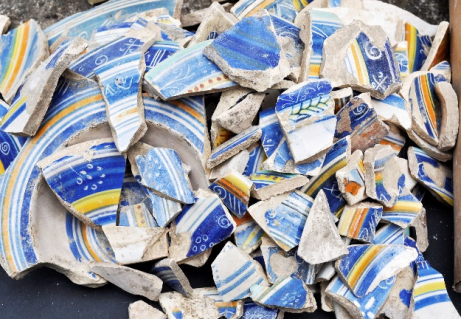
\includegraphics[width=0.45\linewidth]{./picture/material2.png}
		}
		\caption{Material for training}
		\label{2figs}
	\end{figure}
	
	\subsubsection{Label}
	\ 
	
	To get correct and helpful label of categories, the project implements following systems:
	
	\begin{itemize}
		\item A digital comparative collection for pottery types, decorations, and stamps, combining digital collections, digitised paper catalogues, and data acquired through photo campaigns.
		\item A semi-automated system for paper catalogues’ digitisation.
		\item A multilingual thesaurus of descriptive pottery terms, mapped to the Getty Art and Architecture Thesaurus, which includes French, German, Spanish, Catalan, Portuguese, English, and Italian.		
	\end{itemize}
	
	The digital collections and paper catalogues to create digital comparative collections are from already-present databases. 
	
	The first one is ``Roman Amphorae: a digital resource''\cite{Roman_Amphorae}, created by Simon Keay and David Williams of the University of Southampton and published as open data on the Archaeology Data Service, that includes the principal types of roman amphorae between the late 3rd century BCE and the early 7th century CE. The other one is “CERAMALEX” database\cite{CERAMALEX}, a proprietary database of the German and French Heritage 2021.
	
	Limited by space, detailed principles of them will not be shown here.
	
	\subsubsection{Training images}
	\ 
	
	Multiple photo campaigns were also carried out in several archaeological warehouses, involving more than 30 different institutions in Austria, Italy , and Spain. Overall, 3498 sherds were photographed for training the shape-based recognition model. For appearance-based recognition, a dataset of 13,676 pictures was collected through multiple photography campaigns.
	
	To offset disadvantages above in some term, each original image is scaled into four different sizes. On each scaled image, three versions are created: unflipped, horizontally flipped, and vertically flipped. All of these images are cropped, leaving just the central square. As a result, 12 images from each original one were obtained.
	
	
	\subsection{Method}\label{method}
	
	The decoration of pottery fragments have higher priority than shape because decorations is more reliable than the shape of fragments. When decoration presents, decoration will be used to identify rather than appearance. Appearance-based recognition is used only when the pottery is undecorated.
	
	\subsubsection{Shape-based Recognition}
	\ 
	
	The recognition tool was designed as a two-phase process, where the classification algorithm was first developed on one dataset and then validated on other datasets for different types of pottery.
	
	The dataset used 65 standardised toplevel classes defined in Conspectus catalogue\cite{first_phase}. 2D model are created from these drawings and photos taken in archaeological warehouses throughout Europe by extracting the profile of the entire vessel from 2D drawing. Then 2D model rotate around revolution axis to form 3D models.
	
	Then many 3D planes are generated randomly. Computer will calculated how all the circles intersect the plane, connecting the intersection points from the circles along the profile to generate the fracture face. To create a more realistic synthetic fracture, we reduced its size to match real potsherds’ dimensions. \cite{Dellepiane2017FromPT} The progress is shown in Figure \ref{process}.
	
	\begin{figure}[htbp]
		\centering
		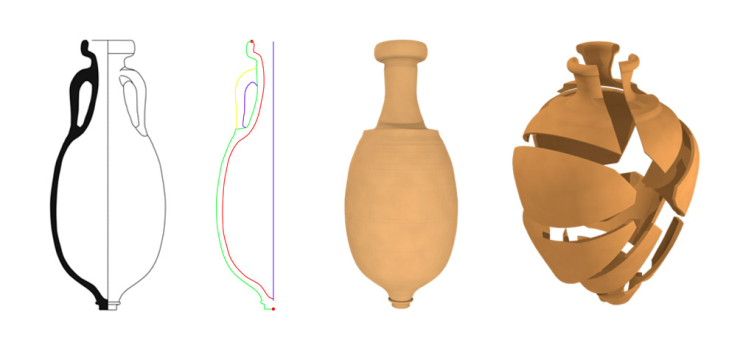
\includegraphics[width=0.5\textwidth]{./picture/process.png}
		\caption{Stpes from extracting profiles from 2D drawings, to creation of 3D models to be broken.}
		\label{process}
	\end{figure} 
	
	The network was trained based on the requirement to divide the inner and the outer profile of the sherd, the relevance of the position of the points along the profile outline, the intrinsic noise in the tracing procedure, and the requirement to overcome sub-optimal data acquisition processes\cite{ANICHINI2021102788}, the example of which is in Figure \ref{process2}.
	
	\begin{figure}[htbp]
		\centering
		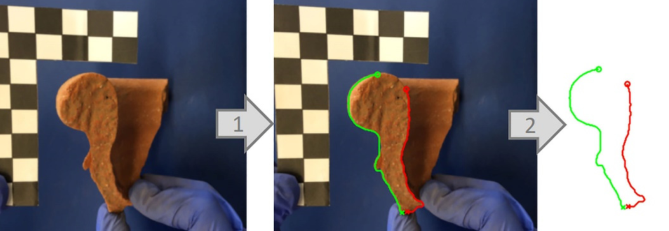
\includegraphics[width=0.5\textwidth]{./picture/fig4.png}
		\caption{Extraction of the outer (green) and inner (red) profiles from image.}
		\label{process2}
	\end{figure} 
	
	To emphasize, the goal is not to increase accuracy of top-1 but that of top-K, which matches straight-forward sense. Because This fits with its function as a reference tool for pottery specialists who would be glad to evaluate a shortlist of results as part of the obligatory expert validation but would be disappointed to use a tool where the correct result is often completely omitted.
	
	\subsubsection{Appearance-based Recognition}
	
	It is find in experience that the most challenging factor that affected identification was varying illumination. So different white balance, brightness, and contrast adjustments are simulated. Each pixel's brightness is multiplied by a random factor to simulate different lighting level.
	
	Moreover, the background and ruler varied significantly, leading to an inherent bias. The foreground was extracted automatically from the training images using the GrabCut algorithm to avoid this conditioning \cite{GrabCut}.
	
	\subsection{App Workflow}\label{workflow}
	
	ArchAIDE also create a mobile application connected to AI classifiers to support archaeologists in recognizing potsherds during excavation and post-excavation analysis, with an easy-to-use interface.
	
	Archaeologists take a picture of a potsherd and send it to the specifically trained classifier, which returns five suggested matches from the comparative collections. Once the correct type is identified, the information is linked to the photographed sherd and stored within a database that can be shared online. As shown in Figure \ref{pic:workflow}.
	
	The mobile application was also designed for allowing the use in lack of internet connectivity , such as in storehouses or remote rural areas. Application provides an area called ``my sites'', dedicated to registered users where it is possible to store information about sites and assemblages. When offline, the app permits storing new images of potsherds or browsing the reference database. The app registers the information locally when offline and then saves the information into the server online.
	
	\begin{figure}[htbp]
		\centering
		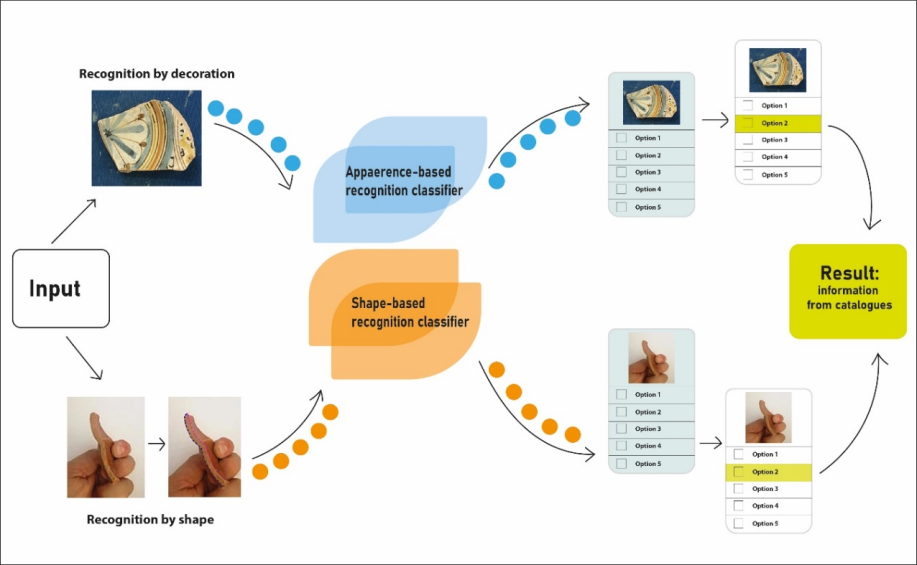
\includegraphics[width=0.5\textwidth]{./picture/workflow.png}
		\caption{The double workflow for appearance-based and shape-based recognition from an input image to top 5 results.}
		\label{pic:workflow}
	\end{figure}  
	
	
	\section{Shortage}
	
	Despite its help, ML still has some limitations.
	
	The biggest difficulty is the shortage of training data. Archaeology is widely digitised, but rarely datafied\cite{Anichini2018BigAD}. ML prefers Big Data which is findable, accessible, interoperable, and reusable. But nature of archaeology makes it hard to produce huge data, and much already-had data is unusable due to copyright or legislation.\cite{heritage4010008}
	
	ML relies on its previously created model too much, and requires new data to be applicable to its model. Most ML models for archaeological data are less reliable than human experts now, because algorithms can't consider the variation and consistencies of data. That is, human experts can quickly handle easy cases, and move extra time to complicate cases, but algorithms handle every sample with same process and consume similar time. This disadvantage may offset ML advantages of high calculation speed and scalability benefits.\cite{bickler_2021}
	
	The diversity of archaeological  objects makes classification more hard. The archaeological recovered samples may become fragmented, or be covered by patina and vegetation. These poor preservation of samples makes classification hard. Moreover, rare and unusual objects may be ignored by ML models. A look-like ``normal'' ceramic vessel may has an unusual surface treatment, which will be easily noticed by human, could be classified into normal category by ML models.\cite{bickler_2021}
	
	A third reason is the accuracy of evaluation function in ML model. This sort of bias is of particular concern for archaeologists using ML on data associated with Indigenous communities. Archaeologists can use surveys based on acultural factors to create models that are stripped of cultural context and meaning. But these assumptions are being more and more challenged, especially when surveys focus on behaviors and outcomes rooted in cultural value systems.\cite{2020_challenge}\cite{2019_challenge}
	

	% needed in second column of first page if using \IEEEpubid
	%\IEEEpubidadjcol

	\section{future}

	Nowadays, archaeologists utilize AI in many ways, from creating 3D models of historical sights
	to scanning territories with a laser radar to find ancient graves or from matching and
	assembling pairs of ancient papyrus fragments containing mostly unknown scripture to detecting
	objects in archaeological sites using DTMs generated from ALS data. There is no denying that 
	AI becomes more and more popular in the field of archaeology and plays an important role in it.

	One direction for the future development of intelligent archaeology is helping archaeologists' work.
	For example, archaeologists often face such problems as not knowing where exactly to dig. 
	They can define the region but not the exact place where an artifact or a grave lies. 
	It's when the neural network comes in line. Instead of looking through millions of documents by themselves, 
	archaeologists pass this work to neural networks. This technology can sort out information by utilizing a 
	specific algorithm. By analyzing images, this system might not only direct archaeologists in their 
	groundworks but also suggest territories that have similar patterns as potential objects for excavations.

	However, knowing that many ML systems --- especially deep neural networks --- are essentially considered black boxes.
	This makes it hard to understand and explain the results given by a model. Because of this, it should be noted that AI does not 
	replace the need for experts in archaeology. Instead, AI technology needs the expertise from archaeologists to improve itself and 
	to judge the correctness of the results.

	Another direction is to strengthen the identification of the artifacts.
	In our world, one of the most urgent problems in archaeology is the fact that
	many artifacts are traded on the dark web. Although 
	many models trained in this direction have achieved 
	quite good results, they are not yet ready to be 
	applied in practice. Currently, the majority of 
	detection operations are performed manually.
	If an AI can succeed in this direction, it would 
	make an extraordinary contribution to the prevention of 
	art-related illegal activities.

	We expect that in the future, artificial intelligence technology will play an increasing, even irreplaceable role in the field of archaeology.
	
	% An example of a floating figure using the graphicx package.
	% Note that \label must occur AFTER (or within) \caption.
	% For figures, \caption should occur after the \includegraphics.
	% Note that IEEEtran v1.7 and later has special internal code that
	% is designed to preserve the operation of \label within \caption
	% even when the captionsoff option is in effect. However, because
	% of issues like this, it may be the safest practice to put all your
	% \label just after \caption rather than within \caption{}.
	%
	% Reminder: the "draftcls" or "draftclsnofoot", not "draft", class
	% option should be used if it is desired that the figures are to be
	% displayed while in draft mode.
	%
	%\begin{figure}[!t]
	%\centering
	%\includegraphics[width=2.5in]{myfigure}
	% where an .eps filename suffix will be assumed under latex, 
	% and a .pdf suffix will be assumed for pdflatex; or what has been declared
	% via \DeclareGraphicsExtensions.
	%\caption{Simulation results for the network.}
	%\label{fig_sim}
	%\end{figure}
	
	% Note that the IEEE typically puts floats only at the top, even when this
	% results in a large percentage of a column being occupied by floats.
	
	
	% An example of a double column floating figure using two subfigures.
	% (The subfig.sty package must be loaded for this to work.)
	% The subfigure \label commands are set within each subfloat command,
	% and the \label for the overall figure must come after \caption.
	% \hfil is used as a separator to get equal spacing.
	% Watch out that the combined width of all the subfigures on a 
	% line do not exceed the text width or a line break will occur.
	%
	%\begin{figure*}[!t]
	%\centering
	%\subfloat[Case I]{\includegraphics[width=2.5in]{box}%
		%\label{fig_first_case}}
	%\hfil
	%\subfloat[Case II]{\includegraphics[width=2.5in]{box}%
		%\label{fig_second_case}}
	%\caption{Simulation results for the network.}
	%\label{fig_sim}
	%\end{figure*}
	%
	% Note that often IEEE papers with subfigures do not employ subfigure
	% captions (using the optional argument to \subfloat[]), but instead will
	% reference/describe all of them (a), (b), etc., within the main caption.
	% Be aware that for subfig.sty to generate the (a), (b), etc., subfigure
	% labels, the optional argument to \subfloat must be present. If a
	% subcaption is not desired, just leave its contents blank,
	% e.g., \subfloat[].
	
	
	% An example of a floating table. Note that, for IEEE style tables, the
	% \caption command should come BEFORE the table and, given that table
	% captions serve much like titles, are usually capitalized except for words
	% such as a, an, and, as, at, but, by, for, in, nor, of, on, or, the, to
	% and up, which are usually not capitalized unless they are the first or
	% last word of the caption. Table text will default to \footnotesize as
	% the IEEE normally uses this smaller font for tables.
	% The \label must come after \caption as always.
	%
	%\begin{table}[!t]
	%% increase table row spacing, adjust to taste
	%\renewcommand{\arraystretch}{1.3}
	% if using array.sty, it might be a good idea to tweak the value of
	% \extrarowheight as needed to properly center the text within the cells
	%\caption{An Example of a Table}
	%\label{table_example}
	%\centering
	%% Some packages, such as MDW tools, offer better commands for making tables
	%% than the plain LaTeX2e tabular which is used here.
	%\begin{tabular}{|c||c|}
	%\hline
	%One & Two\\
	%\hline
	%Three & Four\\
	%\hline
	%\end{tabular}
	%\end{table}
	
	
	% Note that the IEEE does not put floats in the very first column
	% - or typically anywhere on the first page for that matter. Also,
	% in-text middle ("here") positioning is typically not used, but it
	% is allowed and encouraged for Computer Society conferences (but
	% not Computer Society journals). Most IEEE journals/conferences use
	% top floats exclusively. 
	% Note that, LaTeX2e, unlike IEEE journals/conferences, places
	% footnotes above bottom floats. This can be corrected via the
	% \fnbelowfloat command of the stfloats package.
	
	
	
	
	% if have a single appendix:
	%\appendix[Proof of the Zonklar Equations]
	% or
	%\appendix  % for no appendix heading
	% do not use \section anymore after \appendix, only \section*
	% is possibly needed
	
	% use appendices with more than one appendix
	% then use \section to start each appendix
	% you must declare a \section before using any
	% \subsection or using \label (\appendices by itself
	% starts a section numbered zero.)
	%
	

	
	
	% Can use something like this to put references on a page
	% by themselves when using endfloat and the captionsoff option.
	\ifCLASSOPTIONcaptionsoff
	\newpage
	\fi
	
	
	
	% trigger a \newpage just before the given reference
	% number - used to balance the columns on the last page
	% adjust value as needed - may need to be readjusted if
	% the document is modified later
	%\IEEEtriggeratref{8}
	% The "triggered" command can be changed if desired:
	%\IEEEtriggercmd{\enlargethispage{-5in}}
	
	% references section
	
	% can use a bibliography generated by BibTeX as a .bbl file
	% BibTeX documentation can be easily obtained at:
	% http://mirror.ctan.org/biblio/bibtex/contrib/doc/
	% The IEEEtran BibTeX style support page is at:
	% http://www.michaelshell.org/tex/ieeetran/bibtex/
	%\bibliographystyle{IEEEtran}
	% argument is your BibTeX string definitions and bibliography database(s)
	%\bibliography{IEEEabrv,../bib/paper}
	%
	% <OR> manually copy in the resultant .bbl file
	% set second argument of \begin to the number of references
	% (used to reserve space for the reference number labels box)
	\bibliographystyle{acm}
	\bibliography{cited}
	
	% biography section
	% 
	% If you have an EPS/PDF photo (graphicx package needed) extra braces are
	% needed around the contents of the optional argument to biography to prevent
	% the LaTeX parser from getting confused when it sees the complicated
	% \includegraphics command within an optional argument. (You could create
	% your own custom macro containing the \includegraphics command to make things
	% simpler here.)
	%\begin{IEEEbiography}[{\includegraphics[width=1in,height=1.25in,clip,keepaspectratio]{mshell}}]{Michael Shell}
	% or if you just want to reserve a space for a photo:
	
	
	% insert where needed to balance the two columns on the last page with
	% biographies
	%\newpage

	
	% You can push biographies down or up by placing
	% a \vfill before or after them. The appropriate
	% use of \vfill depends on what kind of text is
	% on the last page and whether or not the columns
	% are being equalized.
	
	%\vfill
	
	% Can be used to pull up biographies so that the bottom of the last one
	% is flush with the other column.
	%\enlargethispage{-5in}
	
	
	
	% that's all folks
\end{document}


